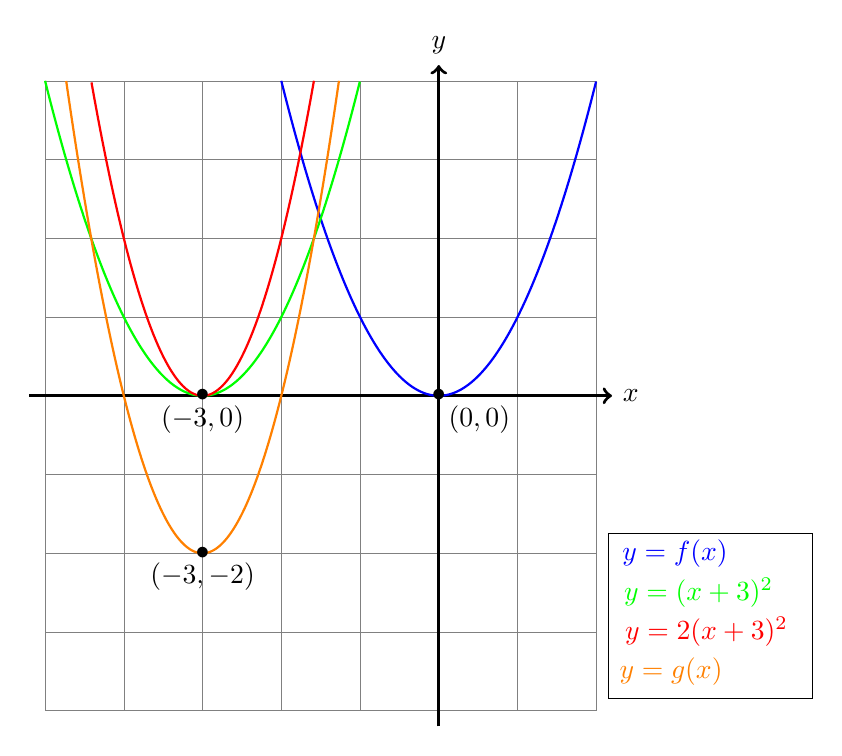
\begin{tikzpicture}
  \draw[very thin,color=gray] (-5,-4) grid (2,4);

  \draw[very thick,->] (-5.2,0) -- (2.2,0) node[right] {$x$};
  \draw[very thick,->] (0,-4.2) -- (0,4.2) node[above] {$y$};
  
  \draw [color=blue,thick] plot[smooth,samples=500,domain=-2:2] (\x,{(\x)^2});
  \draw [color=green,thick] plot[smooth,samples=500,domain=-5:-1] (\x,{(\x + 3)^2});
  \draw [color=red,thick] plot[smooth,samples=500,domain={-3+sqrt(2)}:{-3-sqrt(2)}] (\x,{2*(\x+3)^2});
  \draw [color=orange,thick] plot[smooth,samples=500,domain={-3+sqrt(3)}:{-3-sqrt(3)}] (\x,{2*(\x + 3)^2 - 2});

  \node at (0,0) {$\bullet$};
  \node [below right] at (0,0) {$(0,0)$};
  
  \node at (-3,0) {$\bullet$};
  \node [below] at (-3,0) {$(-3,0)$};

  \node at (-3,-2) {$\bullet$};
  \node [below] at (-3,-2) {$(-3,-2)$};

  %% Legend
  \draw(2.15,-1.75) -- (2.15,-3.85) -- (4.75,-3.85) --( 4.75,-1.75) -- (2.15,-1.75);
  \node [color=blue] at (3,-2)  {$y = f(x)$};
  \node [color=green] at (3.3,-2.5) {$y = (x + 3)^2$};
  \node [color=red] at (3.4,-3) {$y = 2(x+3)^2$};
  \node [color=orange] at (2.95,-3.5) {$y = g(x)$};

\end{tikzpicture}
